% fig03_pipeline.tex — TikZ tabletop accelerator-chain flow diagram for
% §Full Pipeline. Compiled by the paper Makefile via `make figures`
% (pdflatex on the snippet). Tier-color-coded: green = sim/closed-form-PASS
% (closed in this stack), orange = wet-lab / out-of-scope (NOT closed). The
% tier word is inside the node so the diagram is independently readable
% without cross-referencing the §Full Pipeline table.
%
% Manual single-shot compile (debug):
%   pdflatex -interaction=nonstopmode -halt-on-error fig03_pipeline.tex
\documentclass[tikz,border=4pt]{standalone}
\usetikzlibrary{positioning,arrows.meta,shapes.geometric}
\begin{document}
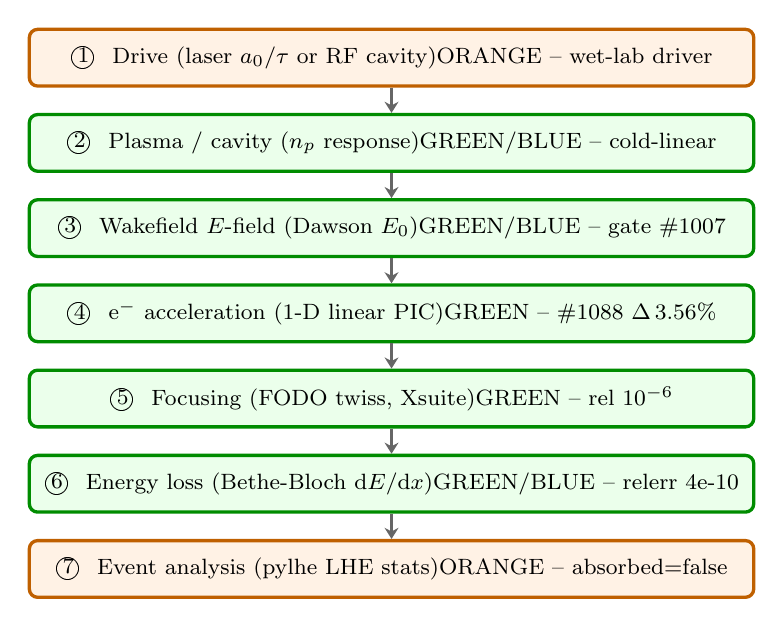
\begin{tikzpicture}[
  font=\footnotesize,
  closed/.style = {
    rectangle, rounded corners=3pt, draw=green!55!black, very thick,
    minimum width=9.2cm, minimum height=0.72cm, align=left,
    fill=green!8,
  },
  wet/.style = {
    rectangle, rounded corners=3pt, draw=orange!75!black, very thick,
    minimum width=9.2cm, minimum height=0.72cm, align=left,
    fill=orange!10,
  },
  arrow/.style = {-{Stealth[length=4pt,width=5pt]}, thick, draw=black!60},
  node distance=0.32cm,
]
  \node[wet]                  (s1)  {\textcircled{1}\ \ Drive (laser $a_0$/$\tau$ or RF cavity)\hfill ORANGE -- wet-lab driver};
  \node[closed, below=of s1]  (s2)  {\textcircled{2}\ \ Plasma / cavity ($n_p$ response)\hfill GREEN/BLUE -- cold-linear};
  \node[closed, below=of s2]  (s3)  {\textcircled{3}\ \ Wakefield $E$-field (Dawson $E_0$)\hfill GREEN/BLUE -- gate \#1007};
  \node[closed, below=of s3]  (s4)  {\textcircled{4}\ \ $\mathrm{e^-}$ acceleration (1-D linear PIC)\hfill GREEN -- \#1088 $\Delta\,3.56\%$};
  \node[closed, below=of s4]  (s5)  {\textcircled{5}\ \ Focusing (FODO twiss, Xsuite)\hfill GREEN -- rel $10^{-6}$};
  \node[closed, below=of s5]  (s6)  {\textcircled{6}\ \ Energy loss (Bethe-Bloch $\mathrm{d}E/\mathrm{d}x$)\hfill GREEN/BLUE -- relerr 4e-10};
  \node[wet,    below=of s6]  (s7)  {\textcircled{7}\ \ Event analysis (pylhe LHE stats)\hfill ORANGE -- absorbed=false};

  \draw[arrow] (s1)  -- (s2);
  \draw[arrow] (s2)  -- (s3);
  \draw[arrow] (s3)  -- (s4);
  \draw[arrow] (s4)  -- (s5);
  \draw[arrow] (s5)  -- (s6);
  \draw[arrow] (s6)  -- (s7);
\end{tikzpicture}
\end{document}
